\chapter{Taming wildlife disease: bridging the gap between science and management}
\chapterauthor{Maxwell B. Joseph, Joseph R. Mihaljevic, Ana Lisette Arellano, Jordan G. Kueneman, Daniel L. Preston, Paul C. Cross, and Pieter T. J. Johnson}
\label{ch1}


Parasites and pathogens of wildlife can threaten biodiversity, infect humans and domestic animals, and cause significant economic losses, providing incentives to manage wildlife diseases. Recent insights from disease ecology have helped transform our understanding of infectious disease dynamics and yielded new strategies to better manage wildlife diseases. Simultaneously, wildlife disease management (WDM) presents opportunities for large-scale empirical tests of disease ecology theory in diverse natural systems.
To assess whether the potential complementarity between WDM and disease ecology theory has been realized, we evaluate the extent to which specific concepts in disease ecology theory have been explicitly applied in peer-reviewed WDM literature.
While only half of WDM articles published in the past decade incorporated disease ecology theory, theory has been incorporated with increasing frequency over the past 40 years. Contrary to expectations, articles authored by academics were no more likely to apply disease ecology theory, but articles that explain unsuccessful management often do so in terms of theory.
Some theoretical concepts such as density-dependent transmission have been commonly applied, whereas emerging concepts such as pathogen evolutionary responses to management, biodiversity–disease relationships and within-host parasite interactions have not yet been fully integrated as management considerations.
Synthesis and applications. Theory-based disease management can meet the needs of both academics and managers by testing disease ecology theory and improving disease interventions. Theoretical concepts that have received limited attention to date in wildlife disease management could provide a basis for improving management and advancing disease ecology in the future.

\section{Why manage wildlife diseases?}

Approximately 43% of emerging human parasites and pathogens originate in wildlife \citep{Jones2008}.
In recent decades, a growing acknowledgement of the role of wildlife diseases in human health has prompted research on pathogens that have directly or indirectly jumped from wildlife to humans, such as human immunodeficiency virus (HIV), severe acute respiratory syndrome (SARS) virus, West Nile virus and various influenza viruses resulting in a rapid increase in the understanding of disease ecology \citep{hudson2002ecology, ostfeld2010infectious, wobeser2013investigation}.
Further impetus for disease ecology research stems from wildlife diseases that afflict domestic animals and cause economic losses due to direct mortality, farm-wide culling and trade restrictions, as seen with classical swine fever, foot-and-mouth disease, bovine tuberculosis and brucellosis \citep{Keeling2001, Schnyder2002, Woodroffe2006, Cross2007b}.

In addition to impacts on human health and economies, wildlife diseases are increasingly recognized as a conservation challenge.
Formerly, it was widely thought that pathogens would not cause extinction because as host population density decreased due to disease, contact rates would become too low for transmission to continue; thus, pathogens would be extirpated before host populations \citep{may1979population}.
However, disease-induced declines and extinctions of wildlife resulting from small population sizes, reservoir hosts, host switching and heterogeneity in contact rates, susceptibility and transmission within and among populations have forced a re-evaluation of this perspective \citep{DeCastro2005b}.
For example, when contact rates among individuals do not depend on host density, pathogens are more likely to drive populations to extinction because transmission continues as host populations are reduced, as seen with Tasmanian devil Sarcophilus harrisii (Boitard 1841) facial tumour disease where transmission appears to be related to mating behaviours \citep{mccallum2012disease}.
White nose syndrome in bats also seems to be more likely to cause extinctions owing to social behaviours in which hosts cluster in hibernacula, reducing the correlation between contact rates and population densities \citep{Langwig2012a}.
In recent decades, wildlife disease management (WDM) has been increasingly used to conserve threatened wildlife populations \citep{Deem2001}.
For example, WDM has controlled outbreaks of feline leukaemia in critically endangered Iberian lynxes Lynx pardinus (Temminck 1827) and rabies in endangered Ethiopian wolves Canis simensis (Rüppell 1840), both of which are associated with domestic animal disease reservoirs \citep{Haydon2006, Lopez2009b}.

Despite the wealth of empirical WDM research, management outcomes can be difficult to predict because system-specific information is lacking for novel pathogens and many theoretical concepts in disease ecology (see Table 1 for a subset) have not been widely tested in the field, leading to uncertainty in their generality.
This is unlike other environmental management disciplines such as fisheries ecology, which has effectively used theoretical models to predict yields, manage harvest timing and limits and design reserves \citep{Gerber2003}.
Indeed, theoretical applications in fisheries ecology have also produced insights into density-dependent population dynamics, metapopulation theory and the evolution of life-history strategies \citep{frank1994fisheries}.
In this review, we assess the extent to which a similar union between theory and practice has been achieved in WDM.

We use a quantitative, case-based approach to provide a critical retrospective of WDM over the last four decades to: (i) quantify how frequently specific theoretical concepts from disease ecology have been applied in the literature, (ii) identify prevailing management objectives, groups and reported outcomes and (iii) assess taxonomic biases in WDM literature. We then present methodological and conceptual opportunities to facilitate the newly emerging synthesis of disease ecology and management, drawing from environmental management and biomedicine to outline steps towards more cost-effective, efficacious and informative WDM. This synthesis aims to facilitate the development of a more predictive framework for disease interventions while simultaneously building empirical support for understanding of disease processes across systems.

\section{Assessing theory application in WDM literature}

\subsection{Systematic search protocol}

We compiled WDM case studies using a systematic, two-step search process with specific criteria for inclusion in our review. In the first stage, we searched titles and abstracts of records included in ISI Web of Science using specific terms [(wild*) AND (disease* OR infect* OR pathogen* OR parasit*) AND (manage* OR conserv*)] to capture breadth in published WDM records.
Additionally, we searched for case studies in grey literature using the following online resources: National Wildlife Health Center, Wildpro, National Biological Information Infrastructure Wildlife Disease Information Node, U.S. Government Printing Office and the U. S. Fish and Wildlife Service.
No case studies identified in the grey literature met our criteria that were independent of cases identified in the scientific literature.
Case studies were also identified using previous review papers and books \citep{Lafferty2002a, wobeser2002, hudson2002ecology, Keesing2006, wobeser2013investigation}.

We conducted a follow-up search with ISI Web of Knowledge to capture subject depth for each managed disease or pathogen identified in the first step, using a search string that included all pathogen and disease names along with terms related to management interventions: (e.g. (rabi* OR lyssavir*) AND (vaccin* OR treat* OR manag* OR control* OR preval* OR incidence OR cull*) AND (wild* OR free-ranging OR free ranging).
The initial Web of Science search returned articles dating back to 1989, but our disease-specific search strings often returned results dating back to the 1950s or earlier.
Historical accounts of WDM are probably under-represented in the literature available online, and those returned by our search strings were often less readily accessible than recently published articles.
As a result, the cases reviewed here primarily represent recently published cases of WDM. The publication dates of included cases range from 1973 to 2011, and 75% of the cases included in our review were published after 1997.

For each article that met our criteria, we recorded (i) pathogen and host characteristics, (ii) management motivations, strategies and outcomes and (iii) whether and how disease ecology theory was incorporated in each article that satisfied our criteria.
We only included cases that provided quantitative data on disease in a population or area (number of cases, seroprevalence, prevalence, incidence, etc.).
When multiple records were encountered for a single management event, we used the most recent record (as of Spring 2011). Cases that only described disease management in humans, livestock or plants were excluded.
Finally, we only included studies that described management of diseases in populations (operationally defined as groups of >1 individual) of free-ranging wildlife.

Incorporation of disease ecology theory was defined broadly as the explicit use or discussion of theoretical concepts relating to transmission dynamics, host population regulation by disease, pathogen evolution, host or pathogen community effects on transmission, spatial heterogeneity in disease dynamics, life stage- or age-specific disease dynamics, endemic vs. epidemic disease states and herd immunity (see Table 1 for a list of specific concepts used to define theory in the literature search).

Four broad management objectives were identified, including conservation of a host species, prevention of disease transmission to humans, prevention of disease transmission to livestock and basic research.
Studies falling into our basic research category were usually an attempt to better understand the system, determine the extent of the disease problem or provide insight into future management opportunities.
To investigate differences in theory application and objectives among managing groups, we also classified author affiliations for each paper as academic, governmental, private or some combination thereof.
University or university laboratory affiliations were considered academic, and we used the same criteria for governmental and private affiliation. Mixed author affiliations (e.g. academic and governmental) were recorded for individual authors and for papers with multiple authors with different affiliations.

We characterized management outcomes by recording whether the disease was eradicated, and if not, whether there were changes in the prevalence, incidence or intensity of disease.
Ideally, these changes could be quantified and compared across disease systems, but in many cases, inconsistent reporting of results and a lack of pre-management or control data complicate meaningful quantitative comparisons of effect sizes across studies.
Finally, we considered whether the original management objective was attained using the following categories: ‘apparent success’, meaning that there was no unmanaged control population or area to compare to the treated area; ‘partial success’, meaning that at least some of the management objectives were reported as fulfilled; and ‘success,’ for cases that had controls and reported fulfillment of all management objectives.
While management outcomes are rarely clear-cut in this practice, this simplified classification system facilitated coarse comparisons across disease systems and among management studies with variable monitoring time-scales.

\section{Results}

In total, 101 scientific articles among the 14 275 identified from the search strings satisfied our criteria.
Many (40%) cases consisted of collaborations between government agencies and academic researchers (Figure \ref{1-1}).
Conservation motivated 87% of management that involved private groups, whereas basic research was only conducted when academics were involved.
Overall, host conservation was the most common objective (39% of cases), while reducing disease risk to humans and domestic animals were the next most common objectives (29% and 24% of cases, respectively; Figure \ref{1-1}).

Disease ecology theory as defined above has only recently been incorporated consistently into WDM literature (Figure \ref{1-2}).
Some theoretical concepts such as density dependence in transmission were frequently applied, while others such as pathogen evolution and the role of predators and biodiversity in regulating disease were not (Figure \ref{1-3}, Table 1).
Unexpectedly, papers authored by academics were not more likely to incorporate theory (Fisher's exact test, P = 0.909).
Management outcomes were related to theory incorporation (Fisher's exact test, P = 0.042).
The three papers that reported disease increases following intervention explained their results in terms of disease ecology theory, providing insights into transmission and optimal control strategies (Figure \ref{1-2}).
However, there was no relationship between management objective attainment and theory incorporation (Fisher's exact test, P = 0.746).
Nevertheless, some counter-intuitive but successful management programmes clearly benefited from theory.
For example, control of classical swine fever in wild boar Sus scrofa (Linnaeus 1758), is often hampered by stage-dependent transmission dynamics. Susceptible piglets are hard to target with baited vaccines and act as disease reservoirs.
By allowing an epidemic to peak such that most adults are immune, then culling only piglets, Swiss academics and governmental groups successfully eradicated the disease from a 166-km2 region near the Italian border \citep{Schnyder2002}.

Reductions in prevalence, incidence or infection intensity were reported in 75% of cases, with vaccination and host treatment as the most commonly applied intervention strategies (Figure \ref{1-2}).
Ninety-four percent of cases reported management in terrestrial systems, with 4% and 2% of cases reporting management in freshwater and marine systems, respectively.
The majority (89%) of reported management efforts were directed towards mammals, with birds and fish representing 10% and 1% of cases, respectively.
However, mammals are less speciose and less threatened by disease than amphibians \citep{vie2009wildlife}, for which we found no published WDM records.
Taxonomic bias could arise because vaccines and drugs are developed primarily to protect human, livestock or poultry health.
Relatively few cases (13%) reported a failure to meet management objectives, possibly due to negative publication bias.

Collectively, our analyses indicate that while academics and government agencies collaborate to manage wildlife diseases, collaborations do not necessarily lead to an integration of disease ecology theory with management.
Density-dependent transmission was often assumed to justify control efforts, but other theoretical concepts were rarely applied (Figure \ref{1-3}).
Data quality issues and potential publication biases currently hinder the application of meta-analytical techniques for WDM, and there is a paucity of published records on non-mammalian management.

\section{Overcoming challenges to theory-based management}

\subsection{Bringing Together Academics and Managers: Obstacles and Opportunities}

While collaboration alone may not necessarily lead to an integration of disease ecology theory and WDM, it should provide a starting point for such integration.
Academics and managers have unique needs, constraints and knowledge-seeking behaviour that challenge such collaborations.
For instance, untreated control areas or pre-treatment data can be unavailable or even unethical in WDM, but are critical for experiments in disease ecology.
While academics may design field experiments to test and refine theoretical models, managers need practical, effective and uncontroversial management strategies that succeed in particular systems.
Such strategies may not be easily identified in the literature from model systems, which managers may be unable to access.

Modelling wildlife disease systems requires decisions about model complexity.
In our experience, theoreticians prefer simpler, more general models that may be applicable to many systems.
These models are easier to parameterize and analyse, and the resulting papers are likely to have a wider academic audience.
On the other hand, simple models are easily discarded by managers because they lack system-specific detail.
This tension is likely to continue, but we recommend additional flexibility on both sides.
In particular, managers should appreciate that the addition of modelling details that are only weakly supported by data may not lead to better predictions.
Meanwhile, theoreticians may develop general models that bear little resemblance to any biological system.
Furthermore, individuals may be most interested in a particular suite of theoretical concepts, but a narrow approach can impede management by ignoring the full range of phenomena relevant to producing desired management outcomes \citep{driscoll2012framework}.
Thus, academics and managers are challenged to take a broad view that incorporates relevant theoretical concepts and an appropriate amount of biological realism, which may require collaboration among researchers with different areas of expertise \citep{driscoll2012framework}.
Unfortunately, such large collaborative efforts may bring a loss of autonomy at odds with academic or governmental bureaucracy.

A diverse body of literature addresses the gap between academics and environmental managers and provides examples of successful strategies for integration.
For instance, international symposia have improved information transfer in invasion biology \citep{Shaw2010a}.
Social networking, joint appointments, interinstitutional sabbaticals, fellowships, concise reporting of relevant science to managers and targeted calls for research proposals by managers can all help to foster cooperation \citep{Gibbons2008}.
Interdisciplinary working groups for particular management issues can ensure that the needs of multiple stakeholders are considered together when organizing such activities \citep{Gibbons2008}.
Groups such as the Wildlife Disease Association and applied journals including the Journal of Wildlife Diseases have encouraged interdisciplinary collaboration, and a broader recognition of the complementarity between disease ecology theory and WDM can provide the impetus for expanding interdisciplinary work in this important field.

\subsection{Meeting the Needs of Managers and Academics}

Theory can help address unprecedented management challenges and can be refined in the process.
Disease outbreaks are often caused by novel pathogens or the appearance of known pathogens in new hosts. Often, details of host–pathogen interactions are unknown.
By combining limited information with general principles of disease ecology (Table 1), management actions can be taken and research priorities identified, informing management as data accumulate \citep{McDonald-Madden2010a}.
Management can test theoretical predictions using large-scale manipulations in real systems, often logistically unfeasible for academics, producing insights and publications even in a crisis.
Field interventions can test concepts of unknown generality in wildlife disease systems.
This is particularly important for management because interventions such as culling are justified on the basis of host density thresholds for disease persistence, which depend on host life-history, seasonality and population dynamics (\cite{Lloyd-Smith2005, altizer2006seasonality}; Figure \ref{1-3}).

Theory is often refined by evaluating competing hypotheses.
Therefore, adaptive management is one way to integrate theory and management, especially if multiple management hypotheses can be tested \citep{holling1978adaptive}.
Differentiation among competing hypotheses is synonymous with identifying optimal management in this framework.
Thus, monitoring the effects of disease interventions on prevalence, virulence and host vital rates can help to estimate model parameters including transmission and recovery rates and help in evaluating management outcomes.
When agencies have limited flexibility in decision-making, thus precluding adaptive management, the best available theoretical and system-specific knowledge can at least produce a ‘best guess’ management strategy \citep{Gregory2006b}.
Failed management is still valuable in this framework because outcomes can be compared to predictions from competing models of disease dynamics that can be selectively eliminated, as with Tasmanian devil facial tumour disease \citep{McDonald-Madden2010a}.
This approach produces mechanistic insights that might be missed if management strategies are characterized simply as effective or ineffective based on management outcomes.

If many groups apply adaptive management separately in similar systems without communicating, generalities that benefit management and disease ecology may remain elusive.
Systematic reviews, invaluable to biomedicine, can help establish which interventions are effective and explain heterogeneity in effectiveness with a standardized meta-analytic approach.
Guidelines for systematic reviews in environmental management exist, but have not been applied in WDM \citep{Pullin2006}.
Our metadata indicate that this may be due to a lack of data quality and quantity.

Simple recommendations to facilitate the production of data suitable in quality for systematic review include: (i) establishing unmanaged control areas and/or baseline data, (ii) achieving replication, (iii) reporting precision for estimates of model parameters, prevalence and effect size, (iv) publishing and mechanistically explaining failed management and (v) reporting the spatiotemporal extent of management.
Data quantity may be lacking because of publication biases and a lack of incentives for managers to publish when working independently.
This latter issue is minor if collaborations involve academics, but even motivated scientists may have difficulty publishing if management has no effect.
However, management failures are as important to report in the literature as successes for systematic reviews and meta-analyses.
An evaluation of the applicability of a theoretical concept in a particular case will rely on comparisons of observed data with explicit predictions from theoretical models, which can often be derived through mathematical modelling.

\subsection{Making Theory Explicit Through Mathematical Modelling}

Theoretical concepts can be explicitly built into system-specific mathematical models to identify and evaluate management strategies, as exemplified in a modern WDM challenge: chronic wasting disease (CWD).
In 2003, the state of Wisconsin began culling white-tailed deer \textit{Odocoileus virginianus} (Zimmermann 1780) and lengthened the hunting season in an attempt to eradicate CWD.
These efforts were mandated despite uncertainty over transmission dynamics, the environmental persistence of prions that cause CWD and the time of CWD arrival to the state \citep{bartelt2003environmental}.
Five years later, prevalence was still slowly increasing \citep{Heisey2010}.
As this epidemic has unfolded, several models have been used to describe the dynamics of CWD \citep{gross2001chronic, Wasserberg2009, wild2011role}.
Simple models of CWD do not tend to produce plausible results.
Purely density-dependent transmission models predict increases in prevalence that are too rapid, while frequency-dependent transmission models predict rapid host extinction or epidemics that are very slow to develop (on the order of centuries).

Modelling indirect transmission via environmental contamination results in a wider range of outcomes and produces several patterns observed in the field including a slow disease progression with prevalences of over 30% and significant host population reduction without rapid extinction \citep{almberg2011modeling}.
Recent analyses did not provide much support for models with variable increases in transmission over models with variable starting prevalence, suggesting that host density effects may be relatively weak in this system \citep{Heisey2010}.
Taken together, these results suggest that managers would have to reduce deer densities to extremely low levels, probably for decades, at which point other stakeholders such as hunters may wonder whether it is worse to have a lower deer density due to disease impacts or disease control efforts.

\subsection{Cautionary Notes and Limitations}

Disease ecology theory is not a ‘silver bullet’ for solving management problems. Indeed, some have pointed out that application of theory under certain circumstances can lead to poor management \citep{driscoll2012framework}.
Misapplication of theory at an inappropriate scale, or in a system that does not meet necessary assumptions, could cause undesired consequences.
For instance, an assumption of broad-scale culling as a disease management intervention is that pathogen transmissions scale positively with host population density.
However, density-dependent changes in social behaviour can alter dispersal patterns that violate this assumption, increasing transmission, as seen with bovine tuberculosis (TB) in cattle and European badgers Meles meles (Linnaeus 1758) \citep{Woodroffe2006}.
Work in the badger–TB system has refined our understanding of the effects of culling on social animals.
However, one could argue that if culling-induced dispersal had been discovered in another disease system, the unintended increase in TB transmission to cattle following badger culling might have been avoided.ons involve academics, but even motivated scientists may have difficulty publishing if management has no effect.
However, management failures are as important to report in the literature as successes for systematic reviews and meta-analyses.
An evaluation of the applicability of a theoretical concept in a particular case will rely on comparisons of observed data with explicit predictions from theoretical models, which can often be derived through mathematical modelling.

\subsection{New Approaches to Reducing Host Susceptibility: Co-infection Dynamics and Probiotics}

Recent advances in disease ecology based on co-infection provide new ways to reduce disease susceptibility and transmission.
For example, in African buffalo \textit{Syncerus caffer} (Sparrman 1779), gastrointestinal nematodes reduce individual resistance to \textit{Mycobacterium tuberculosis}, which causes bovine TB, because of cross-regulatory immune responses to micro- and macroparasites \citep{Ezenwa2010}.
Hence, deworming drugs may increase resistance to TB and improve TB vaccination efficacy, raising the possibility that TB could be managed indirectly through nematode control \citep{Elias2006, Ezenwa2010}.

Management involving immunological trade-offs could improve general understanding of immune-mediated parasite interactions.
For instance, interventions aimed at helminth parasites, which accounted for 25% of cases in our review, are predicted to differentially affect microparasite transmission depending on recovery rates and virulence \citep{Ezenwa2011}.
These predictions could be evaluated opportunistically by monitoring non-target pathogens.
Similarly, management in systems with co-infecting parasites could be used to understand virulence evolution in response to changing co-infection dynamics \citep{Alizon2008c}.

There is increasing recognition that microbial symbiosis can play a role in host health.
Using mutualistic microbes to control disease, a technique known as probiotics therapy, has benefitted aquaculture, agriculture and human medicine.
For example, addition of \textit{Bacillus} and \textit{Pseudomonas} bacteria controls pathogenic Vibrio that infect prawns, salmon and crabs in aquaculture \citep{irianto2002probiotics, panigrahi2007microbial}.
\textit{Bifidobacterium} and \textit{Lactobacillus} can ameliorate \textit{Escherichia coli} infection in pig farms \citep{zani1998effect, shu2001probiotic}.
In humans, probiotics can treat diarrhoea caused by \textit{Clostridium difficile} infection and antibiotic therapy \citep{mcfarland2006meta, rohde2009use}.

Probiotics may prove useful for WDM.
Frogs with certain skin bacteria may be less susceptible to population extirpation caused by chytridiomycosis, a fungal disease that implicated global amphibian declines \citep{Lam2010}.
Experimental augmentation of skin bacteria reduces mortality of susceptible amphibians in captivity, and field experiments are underway to determine whether probiotics can prevent extirpations in nature \citep{Harris2009}.
Probiotics can also reduce vector populations.
For instance, laboratory-reared mosquitoes with a maternally heritable probiotic that disrupts dengue fever virus transmission can locally replace wild mosquito populations and reduce dengue fever risk \citep{hoffmann2011successful}.

The successful use of probiotics depends on an understanding of microbial ecology, especially with respect to long-term probiotic maintenance in a host or environment.
Risks associated with introducing non-native microbes may be ameliorated by isolating probiotic agents from native hosts.
As data accumulate, it will be important to evaluate whether the risks of probiotics outweigh those associated with antibiotic treatment in terms of antibiotic or probiotic resistance and pathogen virulence evolution.
Finally, linking these within-host processes to among-host processes (e.g. microbial community structure and transmission) is an important frontier for WDM and disease ecology.

\subsection{Improving Transmission Interventions in Populations}

Optimal management strategies depend on the degree to which transmission is driven by host population density and the amount of individual and population heterogeneity in contact or transmission rates.
Host population size, aggregation patterns and contact rates can be altered through hunting, artificial feeding, predator and scavenger conservation, fertility control, culling, translocation of individuals, artificial stocking, movement barriers, etc.
Understanding the functional form of the relationships among host contacts, density and transmission in real systems is critical to predicting the impacts of such interventions.
Therefore, field manipulations will play a crucial role in refining our mechanistic understanding of disease transmission.

Optimal management strategies are not static; contact rates, host abundance and demography can change naturally over time, in response to disease and due to management.
For example, group sizes and contact rates may remain constant for highly social species despite management-induced population reduction.
Reservoir hosts may increase disease risk for other species if infected individuals maintain high fitness via increased reproductive output - fecundity compensation, for example \citep{Schwanz2008a}.
Fertility control of such reservoir hosts may protect other species that are less tolerant to infection.
Lastly, if transmission peaks in a short time period, perhaps due to breeding or a pulsed influx of juveniles \citep{altizer2006seasonality}, management may be applied optimally in a narrow time interval.

Brucellosis in the elk (\textit{Cervus elaphus} Linnaeus 1758) populations of the Greater Yellowstone Ecosystem of Wyoming illustrates how management can capitalize on temporal transmission dynamics.
Every year, wildlife managers provide supplemental feed to elk at 22 sites in the region.
Contrary to theoretical predictions, elk abundance at each feeding site is uncorrelated with brucellosis seroprevalence \citep{Cross2007b}, but locally, host contact rates correlate positively with elk density \citep{creech2012effects}.
These seemingly contradictory findings are explained by variation and interaction between transmission and host density over time, which suggests that brucellosis seroprevalence may be reduced by shortening the length of the feeding season in early spring when transmission is highest \citep{maichak2009effects}.
This option is appealing because vaccination has had limited, if any, effect \citep{Cross2007b}, and a test-and-remove programme, although effective, is financially prohibitive to implement across a broad region.

Establishing contact networks for a variety of disease systems across a range of densities and over time will help to identify life-history traits, social structures and other species characteristics that predictably influence transmission.
Taken together, these population-level tools can advance general understanding of transmission dynamics and optimize the application of disease control strategies.

\subsection{Community Matters: Predators, Competitors and Multi-host Parasites}

Community-level interactions including predation and competition can influence disease management outcomes. Predation on hosts can increase or decrease disease prevalence and the likelihood of epidemics depending upon predator selectivity, as well as behavioural and demographic effects on host populations that influence transmission and disease susceptibility \citep{Packer2003, Holt2007}.
Interspecific competition can also influence host background mortality and thus the net effect of disease in a population \citep{bowers1997community}.
Unintended consequences when managing predators or competitors may be of less concern if coupled with ongoing management such as predator restoration and invasive species control.

Interspecific transmission of generalist parasites is hard to quantify, but attempts to control generalist parasites in one host species can reveal the extent to which other hosts contribute to transmission.
For example, vaccinated white-footed mice \textit{Peromyscus leucopus} (Rafinesque 1818) in southern Connecticut reduced the prevalence of \textit{Borrelia burgdorferi}, the bacterium that causes Lyme disease \citep{Tsao2004}.
Based on the strains of \textit{B. burgdorferi} found in ticks in vaccinated plots, and the relationships between mouse density and tick infection prevalence, the authors concluded that other host species contributed more to tick \textit{B. burgdorferi} infections than previously thought.
Thus, vaccination would have to target multiple host species to be effective. Contact prevention between wildlife and livestock also provides an opportunity to prevent disease spillover, and when linked with monitoring of both wildlife and domestic populations, can be used to estimate relative rates of within- and among-species transmission.

Novel management strategies may target ultimate causes of disease emergence once they have been identified.
For instance, Lyme disease risk in the north-eastern United States increases with habitat fragmentation, which leads to extirpations of (i) predators and competitors that limit white-footed mouse abundance and (ii) less-competent hosts for B. burgdorferi and ticks \citep{Ostfeld2003}.
In this system, biodiversity conservation might be an option for proactive WDM. Management interventions that recognize and target community- or ecosystem-level processes are rare, but in some cases may more directly address disease threats than focusing solely on individuals or populations.

\subsection{Evolutionary Responses to Management: A Black Box?}

Common WDM interventions have evolutionary consequences that remain largely unexplored.
In contrast, a vast literature in the biomedical sciences describes the effects of vaccination on the evolution of human pathogens.
Generally, (i) some pathogens tend to evolve vaccine resistance, (ii) imperfect vaccines that confer partial immunity select for increased virulence, and (iii) live attenuated vaccines can revert to virulence if inadequately distributed \citep{anderson1987epidemiology, gandon2007evolutionary, mackinnon2008virulence}.
Together, these observations provide strong incentives for an ‘all or nothing’ approach to vaccine-laden bait distribution programmes, which may jeopardize long-term success if low-coverage field trials using vaccines of limited or unknown efficacy precede full distribution of an effective vaccine.

Selective culling (analogous to selective predation) whereby managers remove infected individuals from the population to prevent disease spread may also have unintended consequences.
It can select for increased virulence, because there are relatively more susceptible hosts available for the pathogen, and pathogens must transmit to susceptible hosts faster to avoid being culled along with their hosts \citep{choo2003host}.
In many cases, selective culls are based on serological tests that do not discriminate between recovered and infectious individuals. Removal of recovered individuals may actually result in more explosive epidemics later on due to a reduction in herd immunity \citep{ebinger2011simulating}.

Experiments and genetic analyses of wildlife pathogens that are often treated by vaccination or culling could reveal the extent to which these concerns are realized.
Aside from developing new vaccines, these risks may be mitigated if management capitalizes on immune-mediated parasite interactions, employ probiotic approaches and consider population- and community-level management interventions.
The use of multiple strategies (seen in 10% of our case studies) may provide one means with which to avoid problems such as antibiotic or vaccine resistance resulting from the overuse of any one strategy.

\section{Conclusions}

A more complete integration of disease ecology with WDM can benefit both disciplines.
Management provides unique opportunities to test disease ecology theory while building system-specific understanding.
By evaluating management outcomes in terms of theory, managers can better identify effective strategies even in the face of management failures.
We have presented specific recommendations, methodological tools and conceptual approaches to achieve a stronger integration of theory and practice, which we hope will facilitate the development of a strong predictive framework for WDM.
The generality of this framework is currently limited by the lack of theoretical and taxonomic breadth of coverage.
However, these biases are beginning to be addressed, and disease ecology theory is being integrated with WDM with increasing frequency. By continuing to incorporate ecological and evolutionary ideas in the development and evaluation of management actions, disease ecology and WDM are likely to continue to advance towards a more unified body of theory and evidence.

\section{Acknowledgements}

We thank Y.P. Springer, V.J. McKenzie, S.H. Paull, S.A. Orlofske, S. Ellis, T.J. Zelikova, the CU Disease Discussion Group and the Johnson Lab for insightful comments.
Any use of trade, product or firm names is for descriptive purposes only and does not imply endorsement by the U.S. Government.
A.L.A., D.L.P., J.G.K., J.R.M. and M.B.J. were supported by the NSF Graduate Research Fellowship Program.
P.C.C.'s work was supported by U.S.G.S. and the NSF/NIH Ecology of Infectious Disease program DEB-1067129, and some ideas stem from working groups sponsored by the NIH/DHS-funded RAPIDD program.
P.T.J.J. was supported by a fellowship from the David and Lucile Packard Foundation and grants from the National Science Foundation (DEB-1149308, 0841758) and the Morris Animal Foundation.


\begin{figure}
	\caption[Management objectives reported in the wildlife disease management literature]{
	Distribution of management objectives across managing groups (G = government agency, A = academic researchers, P = private group, and letter combinations indicate collaborations between groups).
	}
    \begin{center}
	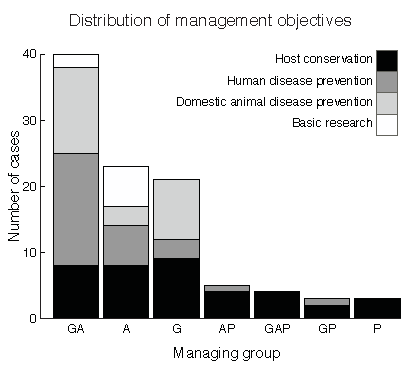
\includegraphics[width=150mm]{figs/ch1/WDMf1.pdf}
    \end{center}
\label{1-1}
\end{figure}

\begin{figure}
	\caption[Temporal trends in the application of theory, and reported management outcome distributions]{
 (a) Time series of theory incorporation in published WDM cases. The size of the dot is proportional to the number of cases included in our review from each time interval. (b) Distribution of management outcomes according to whether disease ecology theory was incorporated. Reductions and increases refer to changes in prevalence, incidence, infection intensity or disease-induced mortality; eradication refers to local rather than global eradication.
	}
    \begin{center}
	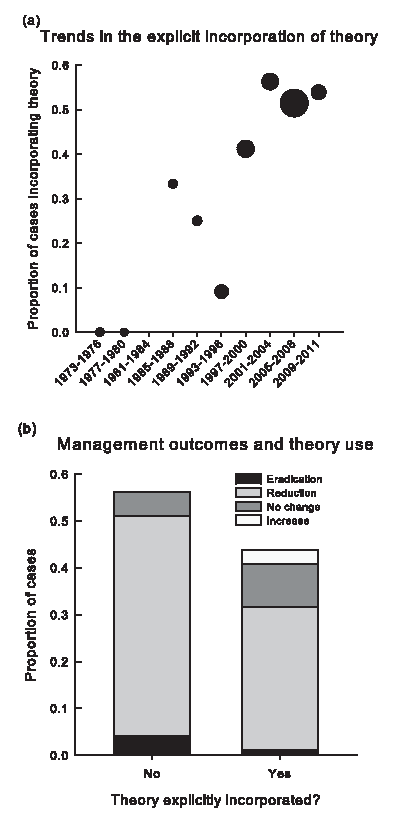
\includegraphics[width=100mm]{figs/ch1/WDMf2.pdf}
    \end{center}
\label{1-2}
\end{figure}


\begin{figure}
	\caption[Theoretical concepts applied in the wildlife disease literature]{
Bar plot of the specific theoretical concepts identified in Table 1, and their application in the literature was included in this review, showing that some concepts such as density-dependent transmission are well represented, while others were less frequently (or not at all) applied.}
    \begin{center}
	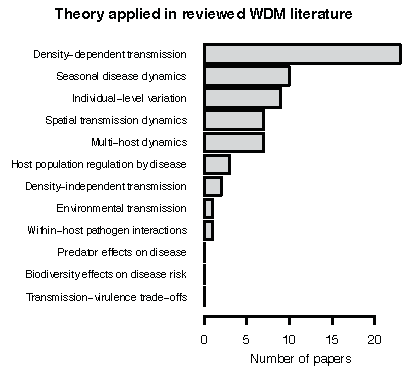
\includegraphics[width=150mm]{figs/ch1/WDMf3.pdf}
    \end{center}
\label{1-3}
\end{figure}

\begin{sidewaystable}
		\centering
		\small
    \caption{
Selected theoretical concepts in disease ecology
	}
    \begin{tabular}{{|p{5cm}|p{12cm}|p{5cm}|}} \hline
	Theoretical concepts & Management applications & Refs. \\  \hline \hline
	Host population regulation by disease & Disease reductions may increase host abundance and/or survival & Anderson and May (1978) \\ \hline
	Trade-offs between transmission and virulence & Artificial stocking may increase virulence, and culling may reduce or increase virulence depending on pathogen life-history, culling selectivity and transmission dynamics & Frank (1996) \\ \hline
	Seasonal drivers of disease emergence and dynamics & Intervention timing and frequency matters; control efforts can target transmission peaks & Altizer et al. (2006) \\ \hline
	Pathogen interactions within hosts & Managing one pathogen alters the transmission and virulence of other pathogens & Fenton (2008) \\ \hline
	Multi-host species disease dynamics	& Reservoir hosts can drive the extinction of alternate hosts; rates of interspecific transmission may be inferred by managing one host species; management may need to target multiple host species & Dobson and Foufopoulos (2001) \\ \hline
	Spread of disease in spatially structured hosts & Corridor vaccination can reduce disease in metapopulations; movement controls are unlikely to work for chronic infections	& Keeling and Eames (2005) \\ \hline
	Transmission increases with host density & Host density reductions may reduce disease transmission, and density thresholds for disease persistence may exist &	Anderson and May (1979) \\ \hline
	Transmission increases with disease prevalence independent of host density & Transmission associated with sexual interactions is more likely to cause host extinction, and non-selective culling may not reduce transmission & Getz and Pickering (1983) \\ \hline
	Predation as a regulator of host population and disease	& Predator conservation may reduce disease in prey populations & Packer et al. (2003) \\ \hline
	Community composition, diversity and disease risk	& Biodiversity loss and community disassembly may increase disease as predators and less-competent hosts are extirpated, depending on community composition and transmission dynamics	& Keesing, Holt and Ostfeld (2006) \\ \hline
	Environmental reservoirs and indirect transmission & Duration of disease control must scale with the environmental persistence; host extinction is more likely	& Joh et al. (2009) \\ \hline
	Individual-level variation and superspreading	& Heterogeneity in individual resistance and infectiousness within a host population can lead to ‘superspreaders’ that account for a large portion of transmission; management can target superspreaders & Lloyd-Smith et al. (2005) \\ \hline
	\end{tabular}
\label{tab1}
\end{sidewaystable}
